\section{Teorema de Fubini}

\subsection{Repaso teórico}
Repasamos ahora los conceptos teóricos necesarios para realizar el cálculo de integrales usando los teoremas de Tonelli y de Fubini. Destacamos estos dos teoremas, que nos ayudan a resolver el cálculo de integrales en varias variables.

\begin{definicion}[Sección de una función]\ \\
    Sea $Z\neq \emptyset $, $f:\mathbb{R}^N\to Z$. Fijado $x\in \mathbb{R}^p$, definimos:
    \begin{equation*}
        f_x:\mathbb{R}^q \to Z \qquad f_x(y) = f(x,y)\quad \forall y\in \mathbb{R}^q
    \end{equation*}
    Análogamente, fijado $y\in \mathbb{R}^q$ se define:
    \begin{equation*}
        f^y:\mathbb{R}^p \to Z \qquad f^y(x) = f(x,y)\quad \forall x\in \mathbb{R}^p
    \end{equation*}
\end{definicion}

\begin{definicion}[Sección de un conjunto]\ \\
    Sea $E\subseteq \mathbb{R}^N$, fijado $x\in \mathbb{R}^p$ definimos:
    \begin{equation*}
        E_x = \{y\in \mathbb{R}^q \mid (x,y)\in E\}
    \end{equation*}
    Análogamente, fijado $y\in \mathbb{R}^q$ definimos:
    \begin{equation*}
        E^y = \{x \in \mathbb{R}^p \mid (x,y)\in E\}
    \end{equation*}
\end{definicion}

\begin{teo}[Teorema de Tonelli]\ \\
    Sea $f:\mathbb{R}^N\to [0,\infty]$ una función \red{medible positiva}, entonces:
    \begin{itemize}
        \item $f_x$ es medible p.c.t. $x\in \mathbb{R}^p$ y $f^y$ es medible p.c.t. $y\in \mathbb{R}^q$.
        \item Las funciones $\varphi$ y $\psi$, definidas c.p.d.\ en $\mathbb{R}^p$ y $\mathbb{R}^q$ respectivamente, por
            \begin{equation*}
                \varphi(x)=\int_{\mathbb{R}^q} f(x,y)dy \text{\ p.c.t.\ }x\in \mathbb{R}^p \qquad \psi(y) = \int_{\mathbb{R}^p} f(x,y)dx \text{\ p.c.t.\ } y \in \mathbb{R}^q
            \end{equation*}
            son medibles y verifican:
            \begin{equation*}
                \int_{\mathbb{R}^N}f(x,y)d(x,y) = \int_{\mathbb{R}^p}\varphi(x)dx = \int_{\mathbb{R}^q}\psi(y)dy
            \end{equation*}
    \end{itemize}
\end{teo}

Por tanto, siempre que tengamos una función \textbf{positiva}, entonces sus integrales iteradas \textbf{coinciden}.\\

La siguiente proposición es consecuencia del Teorema de Tonelli.

\begin{prop}
    Para todo conjunto medible $E\subseteq \mathbb{R}^N$ se tiene:
    \begin{itemize}
        \item $E_x \in \cc{M}_q$ p.c.t. $x\in \mathbb{R}^p$ y $E^y\in \cc{M}_p$ p.c.t. $y\in \mathbb{R}^q$.
        \item Las funciones $x\mapsto \lm_q(E_x)$ e $y\mapsto \lm_p(E^y)$, definidas c.p.d.\ en $\mathbb{R}^p$ y $\mathbb{R}^q$ respectivamente, son medibles con:
            \begin{equation*}
                \lm_N(E) = \int_{\mathbb{R}^p} \lm_q(E_x)dx = \int_{\mathbb{R}^q} \lm_p(E^y)dy
            \end{equation*}
    \end{itemize}
\end{prop}

\begin{teo}[Criterio de integrabilidad]\ \\
    Para $f\in \cc{L}(\mathbb{R}^N)$, se tiene que $f\in \cc{L}_1(\mathbb{R}^N)$ si, y sólo si:
    \begin{equation*}
        \int_{\mathbb{R}^p} \left(\int_{\mathbb{R}^q} |f(x,y)|dy \right)dx<\infty \text{\ o\ bien\ } \int_{\mathbb{R}^q} \left(\int_{\mathbb{R}^p} |f(x,y)|dx\right)dy < \infty
    \end{equation*}
    \begin{proof}
        Como $f$ es medible, sabemos que $|f|$ es una función medible positiva, luego sus integrales iteradas coinciden. Por tanto, si descubrimos que alguna de las dos (que sabemos que son iguales) es finita, sabremos por tanto que $|f|$ es integrable, de donde $f$ también lo será.
    \end{proof}
\end{teo}

\begin{teo}[Teorema de Fubini]
    Sea \red{$f\in \cc{L}_1(\mathbb{R}^N)$}, se tiene:
    \begin{itemize}
        \item $f_x\in \cc{L}_1(\mathbb{R}^q)$ p.c.t. $x\in \mathbb{R}^p$ y $f^y \in \cc{L}_1(\mathbb{R}^p)$ p.c.t. $y\in \mathbb{R}^q$.
        \item Las funciones $\varphi$ y $\psi$ definidas c.p.d.\ en $\mathbb{R}^p$ y $\mathbb{R}^q$ respectivamente, por:
            \begin{equation*}
                \varphi(x)=\int_{\mathbb{R}^q} f(x,y)dy \text{\ p.c.t.\ }x\in \mathbb{R}^p \qquad \psi(y) = \int_{\mathbb{R}^p} f(x,y)dx \text{\ p.c.t.\ } y \in \mathbb{R}^q
            \end{equation*}
            verifican que $\varphi \in \cc{L}_1(\mathbb{R}^p)$ y $\psi \in \cc{L}_1(\mathbb{R}^q)$, con:
            \begin{equation*}
                \int_{\mathbb{R}^N}f(x,y)d(x,y) = \int_{\mathbb{R}^p}\varphi(x)dx = \int_{\mathbb{R}^q}\psi(y)dy
            \end{equation*}
    \end{itemize}
\end{teo}

A pesar de suponer que $f$ era integrable, el teorema nos sirve para probar que ciertas funciones no son integrables, ya que si las integrales iteradas no coinciden o no son menores que infinito, tendremos que la función no es integrable.\\

Finalmente, cabe destacar que si las integrales iteradas coinciden y son finitas y no hemos probado que la función sea integrable, \textbf{no podemos asegurar nada}.


\subsection{Ejercicios}
\begin{ejercicio}
    Probar que el siguiente conjunto es medible y calcular su área.
    \[ E = \left\{ (x, y) \in \mathbb{R}^2 \mid 0 \leq x \leq \min \left\{ e^y , 1 , e^{1-y} \right\} \right\} \subset \mathbb{R}^2 \]

    Tenemos que $E$ es la intersección de tres cerrados, luego $E$ es cerrado y, por tanto, $E\in \cc{M}_2$.
    Para calcular el área de $E$, en primer lugar veamos cuál es el mímino de las tres funciones que definen $E$.
    Tenemos que:
    \begin{align*}
        e^y \leq 1 &\iff e^y \leq e^0 \iff y \leq 0 \\
        e^y \leq e^{1-y} &\iff y \leq 1-y \iff y \leq \nicefrac{1}{2} \\
        e^{1-y} \leq 1 &\iff e^{1-y} \leq e^0 \iff 1-y \leq 0 \iff y \geq 1
    \end{align*}

    Entonces, tenemos que:
    \begin{itemize}
        \item \ul{Si $y \leq 0$}: $e^y \leq 1\leq e^{1-y}$, luego $\min \left\{ e^y , 1 , e^{1-y} \right\} = e^y$.
        \item \ul{Si $0 \leq y \leq \nicefrac{1}{2}$}: $1\leq e^y \leq e^{1-y}$, luego $\min \left\{ e^y , 1 , e^{1-y} \right\} = 1$.
        \item \ul{Si $\nicefrac{1}{2} \leq y \leq 1$}: $1\leq e^{1-y} \leq e^y$, luego $\min \left\{ e^y , 1 , e^{1-y} \right\} = 1$.
        \item \ul{Si $1\leq y$}: $e^{1-y}\leq 1 \leq e^{y}$, luego $\min \left\{ e^y , 1 , e^{1-y} \right\} = e^{1-y}$.
    \end{itemize}

    Por tanto, definimos $f:\bb{R} \to \bb{R}_0^+$ como:
    \[ f(y) = \begin{cases}
        e^y & \text{si } y \leq 0 \\
        1 & \text{si } 0 \leq y \leq 1 \\
        e^{1-y} & \text{si } 1 \leq y
    \end{cases} \]

    Mediante la función $f$ podemos reescribir $E$ como:
    \[ E = \left\{ (x, y) \in \mathbb{R}^2 \mid 0 \leq x \leq f(y) \right\}\in \cc{M}_2 \]

    Visualmente, el conjunto $E$ es el siguiente:
    \begin{figure}[H]
        \centering
        \begin{tikzpicture}
            \begin{axis}[
                domain=-4:6, xmin=-1, xmax=4, ymin=-4, ymax=4,
                samples=100,
                axis lines=center,
                xlabel={$x$},
                ylabel={$y$},
                clip=true,
                axis equal,
                legend cell align=left
            ]
                % Dibuja la curva de y = \ln(x)
                \addplot [name path=A, blue, thick] {ln(x)};
                \addlegendentry{$x=e^y$}

                % Dibuja la curva de y = 1-\ln(x)
                \addplot [name path=B, red, thick] {1-ln(x)};
                \addlegendentry{$x=e^{1-y}$}
            
                % Dibuja la línea vertical en x=1
                \addplot [name path=C, teal, thick] (1,x);
                \addlegendentry{$x=1$}
            
                % Dibuja la línea vertical en x=0
                % \path [name path=D] (axis cs:0,-4) -- (axis cs:0,4);
            
                % Rellena el área bajo la curva entre x=0 y x=1
                \addplot [
                    thick,
                    color=orange,
                    fill=orange,
                    fill opacity=0.4
                ]
                fill between [
                    of=A and B,
                    soft clip={domain=0:1},
                ];
                \addlegendentry{$E$}
            \end{axis}
          \end{tikzpicture}
    \end{figure}

    Como $E$ es la subgráfica de $f$ (función continua, luego medible), entonces el área de $E$ es:
    \begin{equation*}
        \lm_2(E) = \int_{-\infty}^{\infty} f(y)~dy
    \end{equation*}

    Usando la aditividad de la integral, tenemos que:
    \begin{align*}
        \lm_2(E) &= \int_{-\infty}^0 e^y~dy + \int_0^1 1~dy + \int_1^{\infty} e^{1-y}~dy \\
        &= \left[ e^y \right]_{-\infty}^0 + \left[ y \right]_0^1 + \left[ -e^{1-y} \right]_1^{\infty} \\
        &= e^0 - 0 + 1 - 0 - 0 + e^0 = 3
    \end{align*}

    Por tanto, el área de $E$ es $\lm_2(E) = 3$.
\end{ejercicio}

\begin{ejercicio}\label{ej:2.4.2}
    En cada uno de los siguientes casos, probar que la función \( f:\Omega\to \bb{R} \) es integrable en \( \Omega \) y calcular su integral.
    \begin{enumerate}
        \item \(\Omega = \left\{ (x, y) \in \mathbb{R}^2 \mid 0 \leq x \leq 2,~y^2 \leq 2x \right\} \),
        \[ f(x, y) = \frac{x}{\sqrt{1 + x^2 + y^2}} \quad \forall (x, y) \in \Omega \]

        Veamos gráficamente el conjunto $\Omega$:
        \begin{figure}[H]
            \centering
            \begin{tikzpicture}
                \begin{axis}[
                    domain=-1:4, xmin=-1, xmax=8, ymin=-4, ymax=4,
                    samples=100,
                    axis lines=center,
                    xlabel={$x$},
                    ylabel={$y$},
                    clip=true,
                    axis equal,
                    legend cell align=left
                ]
                    % Dibuja la curva de y = \sqrt{2x}
                    \addplot [name path=A, blue, thick, forget plot] {sqrt(2*x)};
                
                    % Dibuja la curva de y = -\sqrt{2x}
                    \addplot [name path=B, blue, thick] {-sqrt(2*x)};
                    \addlegendentry{$x=\nicefrac{y^2}{2}$}
                
                    % Dibuja la línea vertical en x=2
                    \addplot [name path=C, teal, thick] (2,-4) -- (2,4);
                    \addlegendentry{$x=2$}
                
                    % Rellena el área bajo la curva entre x=0 y x=2
                    \addplot [
                        thick,
                        color=orange,
                        fill=orange,
                        fill opacity=0.4
                    ]
                    fill between [
                        of=A and B,
                        soft clip={domain=0:2},
                    ];
                    \addlegendentry{$\Omega$}
                \end{axis}
              \end{tikzpicture}
        \end{figure}

        El conjunto $\Omega$ es la intersección de tres cerrados, luego $\Omega$ es cerrado y, por tanto, $\Omega\in \cc{M}_2$.
        Además, este se puede expresar como:
        \[ \Omega = \left\{ (x, y) \in \mathbb{R}^2 \mid 0 \leq x \leq 2,|x| \leq \sqrt{2x} \right\} \]

        Veamos en primer lugar que $\Omega$ está acotado. Sabemos que es medible por ser intersección de cerrados, y está acotado ya que
        para todo $(x, y) \in \Omega$ se tiene que:
        \begin{equation*}
            |x|\leq 2
            \hspace{2cm}
            |y|\leq \sqrt{2x} \leq \sqrt{2\cdot 2} = 2
        \end{equation*}

        Por tanto, $\lm_2(\Omega) \leq 4^2 < \infty$. Tenemos además que $f$ es continua, luego medible. Veamos que está acotada:
        \begin{equation*}
            |f(x,y)| = \left| \frac{x}{\sqrt{1 + x^2 + y^2}} \right| \leq |x| \leq 2
            \qquad \forall (x, y) \in \Omega
        \end{equation*}

        Por tanto, veamos que $f$ es integrable en $\Omega$:
        \begin{equation*}
            \int_{\Omega} |f(x, y)|~d(x, y) \leq \int_{\Omega} 2~d(x, y) = 2 \lm_2(\Omega) < \infty
        \end{equation*}

        Por tanto, tenemos que $f\in \cc{L}_1(\Omega)$. Calculemos ahora las secciones verticales y horizontales:
        \begin{align*}
            \Omega_x &= \emptyset \qquad \forall x \in \mathbb{R} \setminus [0, 2] \\
            \Omega_x &= \left[ -\sqrt{2x}, \sqrt{2x} \right] \qquad \forall x \in [0, 2] \\
            \Omega_y &= \emptyset \qquad \forall y \in \mathbb{R} \setminus [-2, 2] \\
            \Omega_y &= \left[ \dfrac{y^2}{2}, 2\right] \qquad \forall y \in [-2, 2]
        \end{align*}
        
        
        Por el Teorema de Fubini, tenemos que:
        \begin{align*}
            \int_{\Omega} f(x, y)~d(x, y)
            &= \int_{0}^{2} \left( \int_{-\sqrt{2x}}^{\sqrt{2x}} \frac{x}{\sqrt{1 + x^2 + y^2}}~dy \right)~dx\\
            &= \int_{-2}^{2} \left( \int_{\frac{y^2}{2}}^{2} \frac{x}{\sqrt{1 + x^2 + y^2}}~dx \right)~dy
        \end{align*}

        Como vemos, el Teorema de Fubini nos permite calcular la integral de $f$ en $\Omega$ de dos formas distintas. No obstante,
        la segunda es más sencilla, ya que la integral interna es más sencilla de calcular. Por tanto, optamos por esta última:
        \begin{align*}
            \int_{\Omega} f(x, y)~d(x, y)
            &= \int_{-2}^{2} \left( \int_{\frac{y^2}{2}}^{2} \frac{x}{\sqrt{1 + x^2 + y^2}}~dx \right)~dy \\
            &= \int_{-2}^{2} \left[ \sqrt{1 + x^2 + y^2} \right]_{\frac{y^2}{2}}^{2}~dy \\
            &= \int_{-2}^{2} \left( \sqrt{1 + 4 + y^2} - \sqrt{1 + \frac{y^4}{4} + y^2} \right)~dy \\
            &= \int_{-2}^{2} \left( \sqrt{5 + y^2} -  \sqrt{\left(\frac{y^2}{2}+1\right)^2} \right)~dy \\
            &= \int_{-2}^{2} \left( \sqrt{5 + y^2} -  \frac{y^2}{2} -1 \right)~dy
        \end{align*}

        Buscamos ahora resolver la integral de la raíz cuadrada. Tenemos que:
        \begin{align*}
            \int_{-2}^{2} \sqrt{5 + y^2}~dy
            &= \sqrt{5}\int_{-2}^{2} \sqrt{1 + \left(\frac{y}{\sqrt{5}}\right)^2}~dy
        \end{align*}

        Hay dos cambios de variable posibles para resolver esta integral.
        \begin{description}
            \item[Opción 1.] Cambio de variable trigonométrico:
            
            Sea el intervalo $I=\left[-\arctan\left(\nicefrac{2}{\sqrt{5}}\right), \arctan\left(\nicefrac{2}{\sqrt{5}}\right)\right]$, 
            que por comodidad lo denotaremos como $I=[-\alpha, \alpha]$. Definimos $\varphi:I \to \mathbb{R}$ como
            $\varphi(t)=\sqrt{5}\tg(t)$. Entonces, tenemos que $\varphi\in C^1(I)$, $\varphi(I)=[-2,2]$ y $\varphi'(t)=\sqrt{5}\sec^2(t)\neq 0$ en $I$. Por tanto,
            por el Teorema de Cambio de Variable, tenemos que:
            \begin{align*}
                \int_{-2}^{2} \sqrt{5 + y^2}~dy
                &= \sqrt{5}\int_{-\alpha}^{\alpha} \sqrt{1 + \left(\frac{\sqrt{5}\tg(t)}{\sqrt{5}}\right)^2}\sqrt{5}\sec^2(t)~dt \\
                &= 5\int_{-\alpha}^{\alpha} \sqrt{1 + \tg^2(t)}\sec^2(t)~dt \\
                &= 5\int_{-\alpha}^{\alpha} \sec^3(t)~dt
            \end{align*}

            Para resolver esta integral, usamos el método de Integración por Partes.
            Sean $F,G:I\to\mathbb{R}$ definidas como $F(t)=\sec(t)$ y $G(t)=\tg(t)$. Entonces, tenemos que $F,G\in C^1(I)$, por lo que:
            \begin{align*}
                \int_{-\alpha}^{\alpha} \sec^3(t)~dt
                &= \left[ \sec(t)\tg(t) \right]_{-\alpha}^{\alpha} - \int_{-\alpha}^{\alpha} \tg(t)\sec(t)\tg(t)~dt \\
                &= \left[ \sec(t)\tg(t) \right]_{-\alpha}^{\alpha} - \int_{-\alpha}^{\alpha} \sec(t)\tg^2(t)~dt \\
                &= \left[ \sec(t)\tg(t) \right]_{-\alpha}^{\alpha} - \int_{-\alpha}^{\alpha} \sec(t)(\sec^2(t)-1)~dt \\
                &= \left[ \sec(t)\tg(t) \right]_{-\alpha}^{\alpha} - \int_{-\alpha}^{\alpha} \sec^3(t)~dt + \int_{-\alpha}^{\alpha} \sec(t)~dt
            \end{align*}

            Despejando la integral que queremos calcular, tenemos que:
            \begin{align*}
                2\int_{-\alpha}^{\alpha} \sec^3(t)~dt
                &= \left[ \sec(t)\tg(t) \right]_{-\alpha}^{\alpha} + \int_{-\alpha}^{\alpha} \sec(t)\cdot \frac{\sec(t)+\tg(t)}{\sec(t)+\tg(t)}~dt \\
                &= \left[ \sec(t)\tg(t) \right]_{-\alpha}^{\alpha} + \int_{-\alpha}^{\alpha} \frac{\sec^2(t)+\sec(t)\tg(t)}{\sec(t)+\tg(t)}~dt \\
                &= \left[ \sec(t)\tg(t) \right]_{-\alpha}^{\alpha} + \left[ \ln|\sec(t)+\tg(t)| \right]_{-\alpha}^{\alpha} \\
                &= \tg(\alpha) \left(\sec(\alpha)-\sec(-\alpha)\right) +  \ln\left|\dfrac{\sec(\alpha)+\tg(\alpha)}{\sec(-\alpha)+\tg(-\alpha)}\right| \\
                &= 2\tg(\alpha)\sec(\alpha) + \ln\left|\dfrac{\sec(\alpha)+\tg(\alpha)}{\sec(-\alpha)+\tg(-\alpha)}\right| \\
                &= 2\tg(\alpha)\sec(\alpha) + \ln\left|\dfrac{\sec(\alpha)+\tg(\alpha)}{\sec(\alpha)-\tg(\alpha)}\right|
            \end{align*}

            Veamos ahora cuánto vale $\sec(\alpha)$. Tenemos que:
            \begin{equation*}
                \tg^2(\alpha) + 1 = \sec^2(\alpha) = \frac{4}{5} + 1 = \frac{9}{5}
                \Longrightarrow \sec(\alpha) = \sqrt{\frac{9}{5}} = \frac{3}{\sqrt{5}}
            \end{equation*}
            
            Por tanto, tenemos que:
            \begin{align*}
                \int_{-\alpha}^{\alpha} \sec^3(t)~dt
                &= \tg(\alpha)\sec(\alpha) + \frac{1}{2}\ln\left|\dfrac{\sec(\alpha)+\tg(\alpha)}{\sec(\alpha)-\tg(\alpha)}\right| \\
                &= \frac{2}{\sqrt{5}}\cdot \frac{3}{\sqrt{5}} + \frac{1}{2}\ln\left|\dfrac{\frac{3}{\sqrt{5}}+\frac{2}{\sqrt{5}}}{\frac{3}{\sqrt{5}}-\frac{2}{\sqrt{5}}}\right| \\
                &= \frac{6}{5} + \frac{1}{2}\ln\left|\dfrac{\frac{5}{\sqrt{5}}}{\frac{1}{\sqrt{5}}}\right| = \frac{6}{5} + \frac{1}{2}\ln(5) \\
            \end{align*}

            Retrocediendo en las integrales, tenemos que:
            \begin{align*}
                \int_{-2}^{2} \sqrt{5 + y^2}~dy
                &= 5\int_{-\alpha}^{\alpha} \sec^3(t)~dt \\
                &= 5\left( \frac{6}{5} + \frac{1}{2}\ln(5) \right) = 6 + \frac{5}{2}\ln(5)
            \end{align*}

            \item[Opción 2.] Cambio de variable con funciones hiperbólicas:
            
            Sea ahora la función $\varphi:\bb{R}\to \bb{R}$ definida como:
            \[ \varphi(t) = \sqrt{5}\senh(t) = \sqrt{5}\left( \frac{e^t - e^{-t}}{2} \right) \]

            Entonces, tenemos que $\varphi\in C^1(\bb{R})$ y como la función a integrar es continua en $\bb{R}$, podemos aplicar la versión elemental del Teorema de Cambio de Variable. Calculemos los nuevos límites de integración:
            \begin{align*}
                \varphi(t) = 2 &\iff \sqrt{5}\senh(t) = 2 \iff \senh(t) = \frac{2}{\sqrt{5}} \iff e^t - e^{-t} = \frac{4}{\sqrt{5}} \\
                &\iff e^{2t} - 1 = \frac{4}{\sqrt{5}}e^t \iff e^{2t} - \frac{4}{\sqrt{5}}e^t - 1 = 0 \\
                &\iff e^t=\sqrt{5} \iff t = \ln(\sqrt{5}) = \frac{\ln(5)}{2}
            \end{align*}

            Como la función es impar, sabemos que $\varphi\left(-\frac{\ln(5)}{2}\right) = -2$. Por tanto, por el Teorema de Cambio de Variable, tenemos que:
            \begin{align*}
                \int_{-2}^{2} \sqrt{5 + y^2}~dy
                &= \sqrt{5}\int_{-\frac{\ln(5)}{2}}^{\frac{\ln(5)}{2}} \sqrt{1+\senh^2(t)}\cosh(t)~dt \\
                &= 5\int_{-\frac{\ln(5)}{2}}^{\frac{\ln(5)}{2}} \cosh^2(t)~dt
            \end{align*}

            Usando relaciones trigonométricas, tenemos que:
            \begin{equation*}
                \left\{
                    \begin{aligned}
                        \cosh^2(t) - \senh^2(t) &= 1 \\
                        \cosh^2(t) + \senh^2(t) &= \cosh(2t)
                    \end{aligned}
                \right\} \Longrightarrow
                \cosh^2(t) = \frac{1+\cosh(2t)}{2}
            \end{equation*}

            Por tanto, tenemos que:
            \begin{align*}
                \int_{-2}^{2} \sqrt{5 + y^2}~dy
                &= 5\int_{-\frac{\ln(5)}{2}}^{\frac{\ln(5)}{2}} \frac{1+\cosh(2t)}{2}~dt \\
                &= \frac{5}{2}\left[ t + \frac{\senh(2t)}{2} \right]_{-\frac{\ln(5)}{2}}^{\frac{\ln(5)}{2}} \\
                &= \frac{5}{2}\left( \frac{\ln(5)}{2} + \frac{\senh(\ln(5))}{2} + \frac{\ln(5)}{2} - \frac{\senh(-\ln(5))}{2} \right) \\
                &= \frac{5}{2}\left( \ln(5) + \frac{e^{\ln(5)} - e^{-\ln(5)}}{4} - \frac{e^{-\ln(5)} - e^{\ln(5)}}{4} \right) \\
                &= \frac{5}{2}\left( \ln(5) + \frac{5 - \nicefrac{1}{5}}{4} - \frac{\nicefrac{1}{5} - 5}{4} \right) \\
                &= \frac{5}{2}\left( \ln(5) + \frac{12}{5}\right)
                = 6 + \frac{5}{2}\ln(5)
            \end{align*}
        \end{description}

        \begin{observacion}
            El lector posiblemente no esté familiarizado con las funciones hiperbólicas, y por ello
            podría pensar en optar por la primera opción. No obstante, la segunda opción es más sencilla,
            ya que el cálculo de la integral de $\sec^3(t)$ es más complejo. No obstante,
            optamos por dejar ambas opciones para que el lector se familiarice con las funciones hiperbólicas y,
            de igual forma, conozca cómo calcular la integral de $\sec^3(t)$, que es una integral que,
            sin haberla leído antes, puede resultar complicada.
        \end{observacion}
        

        En cualquier caso, tenemos que:
        \begin{align*}
            \int_{\Omega} f(x, y)~d(x, y)
            &= \int_{-2}^{2} \left( \sqrt{5 + y^2} -  \frac{y^2}{2} -1 \right)~dy \\
            &= 6 + \frac{5}{2}\ln(5) - \int_{-2}^{2} \frac{y^2}{2}~dy - \int_{-2}^{2} 1~dy \\
            &= 6 + \frac{5}{2}\ln(5) - \left[ \frac{y^3}{6} \right]_{-2}^{2} - \left[ y \right]_{-2}^{2} \\
            &= 6 + \frac{5}{2}\ln(5) - \frac{8}{6} - \frac{8}{6} -2 -2 \\
            &= 6 + \frac{5}{2}\ln(5) - \frac{8}{3} - 4 = \frac{5}{2}\ln(5) - \frac{2}{3}
        \end{align*}

        \item \label{ej:2.4.2.2} \(\Omega = \left\{ (x, y) \in \mathbb{R}^2 \mid x^2 + y^2 \leq 1,~x^2 + y^2 \leq 2x \right\} \),
        \[ f(x, y) = x \quad \forall (x, y) \in \Omega \]

        Veamos en primer lugar cómo es el conjunto $\Omega$. Tenemos que:
        \begin{equation*}
            x^2 + y^2 \leq 2x \iff
            x^2 - 2x + 1 + y^2 \leq 1 \iff
            (x-1)^2 + y^2 \leq 1
        \end{equation*}

        Por tanto, tenemos que $\Omega$ gráficamente es:
        \begin{figure}[H]
            \centering
            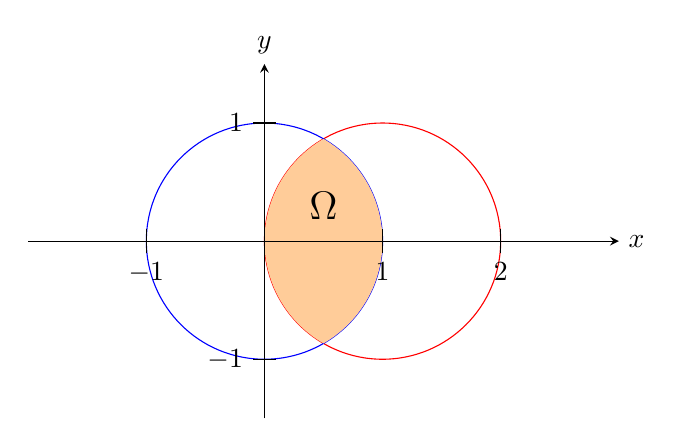
\begin{tikzpicture}[scale=1.5]
                % Dibuja las dos circunferencias
                \draw[red] (1,0) circle (1);
                \draw[blue] (0,0) circle (1);
                
                % Rellena la intersección de las dos circunferencias
                \begin{scope}
                    \clip (1,0) circle (1);
                    \fill[orange!40] (0,0) circle (1);
                    \node at (0.5,0.3) {{\Large$\Omega$}};
                \end{scope}
                
                % Dibuja los ejes
                \draw[-stealth] (-2,0) -- (3,0) node[right] {$x$};
                \draw[-stealth] (0,-1.5) -- (0,1.5) node[above] {$y$};

                % Marcas en los ejes
                \foreach \x in {-1,1,2}
                    \draw (\x,0.1) -- (\x,-0.1) node[below] {$\x$};
                \foreach \y in {-1,1}
                    \draw (0.1,\y) -- (-0.1,\y) node[left] {$\y$};
            \end{tikzpicture}
        \end{figure}

        El conjunto $\Omega$ es la intersección de dos cerrados, luego $\Omega$ es cerrado y, por tanto, $\Omega\in \cc{M}_2$.
        Además, como $|x|\leq 1$ y $|y|\leq 1$, entonces $\Omega$ está acotado, con $\lm_2(\Omega)\leq 2^2 < \infty$.
        Por otro lado, la función $f$ es continua, luego medible. Veamos que $f$ es integrable en $\Omega$:
        \begin{equation*}
            \int_{\Omega} |f(x, y)|~d(x, y)
            = \int_{\Omega} |x|~d(x, y) \leq \int_{\Omega} 1~d(x, y) = \lm_2(\Omega) < \infty
        \end{equation*}

        Por tanto, $f\in \cc{L}_1(\Omega)$. Calculemos ahora las secciones verticales.
        Tenemos que:
        \begin{equation*}
            y^2\leq 1-x^2 \hspace{1cm} y^2\leq 2x-x^2
        \end{equation*}

        Veamos qué valor es menor en cada caso:
        \begin{equation*}
            1-x^2 \leq 2x-x^2 \iff 1 \leq 2x \iff \frac{1}{2} \leq x
        \end{equation*}

        Calculemos ahora las secciones verticales. Como $x^2\leq 1$ y $(x-1)^2\leq 1$, entonces tenemos que
        $x\in [0,1]$. Por tanto, para $x\in \bb{R}\setminus [0,1]$ tenemos que $\Omega_x=\emptyset$, en caso contrario:
        \begin{itemize}
            \item Si $x\in [0,\nicefrac{1}{2}]$, entonces $y^2\leq 2x-x^2$, por lo que:
            \begin{equation*}
                \Omega_x = \left[ -\sqrt{2x-x^2}, \sqrt{2x-x^2} \right]
            \end{equation*}

            \item Si $x\in [\nicefrac{1}{2},1]$, entonces $y^2\leq 1-x^2$, por lo que:
            \begin{equation*}
                \Omega_x = \left[ -\sqrt{1-x^2}, \sqrt{1-x^2} \right]
            \end{equation*}
        \end{itemize}
        
        Por el Teorema de Fubini, tenemos que:
        \begin{align*}
            \int_{\Omega} f(x, y)~d(x, y) &= \int_{0}^{1} \left( \int_{\bb{R}} f(x,y)~dy \right)~dx =\\
            &= \int_{0}^{\nicefrac{1}{2}} \left( \int_{-\sqrt{2x-x^2}}^{\sqrt{2x-x^2}} x~dy \right)~dx +
            \int_{\nicefrac{1}{2}}^{1} \left( \int_{-\sqrt{1-x^2}}^{\sqrt{1-x^2}} x~dy \right)~dx
        \end{align*}

        Resolvamos ahora las integrales internas:
        \begin{align*}
            \int_{-\sqrt{2x-x^2}}^{\sqrt{2x-x^2}} x~dy
            &= x\left[ y \right]_{-\sqrt{2x-x^2}}^{\sqrt{2x-x^2}} = x\left( \sqrt{2x-x^2} - (-\sqrt{2x-x^2}) \right) = 2x\sqrt{2x-x^2} \\ \\
            \int_{-\sqrt{1-x^2}}^{\sqrt{1-x^2}} x~dy
            &= x\left[ y \right]_{-\sqrt{1-x^2}}^{\sqrt{1-x^2}} = x\left( \sqrt{1-x^2} - (-\sqrt{1-x^2}) \right) = 2x\sqrt{1-x^2}
        \end{align*}

        Calculemos ahora las integrales externas. Para la primera integral, tenemos que:
        \begin{align*}
            \int_{0}^{\nicefrac{1}{2}} 2x\sqrt{2x-x^2}~dx
            &= \int_{0}^{\nicefrac{1}{2}} 2x\sqrt{1-(x-1)^2}~dx
        \end{align*}
        
        Sea ahora la función $\varphi:[0, \pi]\to\bb{R}$ definida como $\varphi(t)=\cos(t)+1$. Entonces, tenemos que $\varphi\in C^1([0,1])$,
        y además $\varphi(\pi) = 0$ y $\varphi\left(\frac{2\pi}{3}\right) = \nicefrac{1}{2}$.
        Por tanto, por el Teorema de Cambio de Variable, tenemos que:
        \begin{align*}
            \int_{0}^{\nicefrac{1}{2}} &2x\sqrt{1-(x-1)^2}~dx
            = \int_{\pi}^{\frac{2\pi}{3}} 2\left(\cos(t)+1\right)\sen(t)\cdot (-\sen(t))~dt \\
            &= -2\int_{\pi}^{\frac{2\pi}{3}} \left(\cos(t)+1\right)\sen^2(t)~dt
            = -2\int_{\pi}^{\frac{2\pi}{3}} \cos(t)\sen^2(t)~dt - 2\int_{\pi}^{\frac{2\pi}{3}} \sen^2(t)~dt \\
            &= -2\left[\dfrac{\sen^3(t)}{3}\right]_{\pi}^{\frac{2\pi}{3}} - 2\int_{\pi}^{\frac{2\pi}{3}} \dfrac{1-\cos(2t)}{2}~dt
            = -\frac{2}{3}\left[\sen^3(t)\right]_{\pi}^{\frac{2\pi}{3}} - \left[t-\dfrac{\sen(2t)}{2}\right]_{\pi}^{\frac{2\pi}{3}} \\
            &= -\frac{2}{3}\left(\sen^3\left(\frac{2\pi}{3}\right)-\sen^3(\pi)\right) - \left(\frac{2\pi}{3}-\frac{\sen\left(\frac{4\pi}{3}\right)}{2}-\pi+\frac{\sen(2\pi)}{2}\right) \\
            &= -\frac{\sqrt{3}}{4} +\frac{\pi}{3}-\frac{\sqrt{3}}{4} = \frac{\pi}{3}-\frac{\sqrt{3}}{2}
        \end{align*}

        Para la segunda integral, definimos $\psi:[0, \pi]\to\bb{R}$ como $\psi(t)=\cos(t)$. Entonces, tenemos que $\psi\in C^1([0,1])$,
        y además $\psi(0) = 1$ y $\psi\left(\frac{\pi}{3}\right) = \nicefrac{1}{2}$. Por tanto, por el Teorema de Cambio de Variable, tenemos que:
        \begin{align*}
            \int_{\nicefrac{1}{2}}^{1} &2x\sqrt{1-x^2}~dx
            = \int^{0}_{\frac{\pi}{3}} 2\cos(t)\sen(t)\cdot (-\sen(t))~dt
            = -2\int^{0}_{\frac{\pi}{3}} \cos(t)\sen^2(t)~dt \\
            &= -2 \left[\dfrac{\sen^3(t)}{3}\right]^{0}_{\frac{\pi}{3}}
            = -\frac{2}{3}\left(\sen^3(0)-\sen^3\left(\frac{\pi}{3}\right)\right) = \frac{\sqrt{3}}{4}
        \end{align*}

        Por tanto, tenemos que:
        \begin{align*}
            \int_{\Omega} f(x, y)~d(x, y)
            &= \int_{0}^{\nicefrac{1}{2}} 2x\sqrt{2x-x^2}~dx + \int_{\nicefrac{1}{2}}^{1} 2x\sqrt{1-x^2}~dx \\
            &= \frac{\pi}{3}-\frac{\sqrt{3}}{2} + \frac{\sqrt{3}}{4} = \frac{\pi}{3}-\frac{\sqrt{3}}{4}
        \end{align*}

        \begin{observacion}
            Notemos que, en este ejercicio, no habría sido necesario demostrar que $f\in \cc{L}_1(\Omega)$ demostrando
            que $f$ y $\Omega$ son acotadas. Como se tiene que $f(x,y)=x\geq 0$ para todo $(x,y)\in \Omega$, entonces
            podríamos haber trabajado con la integral definida para $\cc{L}^+(\bb{R}^2)$, y al ver que
            esta integral es finita, como $|f|=f$, entonces $f\in \cc{L}_1(\Omega)$.
            No obstante, para acostumbrarnos al otro proceso, se ha optado por la primera forma. Esta segunda opción se trabajará en el siguiente ejercicio.
        \end{observacion}

        \item \(\Omega = \left\{ (x, y, z) \in \mathbb{R}^3 \mid 0 < x < y < z \right\} \),
        \[ f(x, y, z) = e^{-(x+y+z)} \quad \forall (x, y, z) \in \Omega \]

        El conjunto $\Omega$ es un abierto por ser la intersección de tres abiertos, luego $\Omega\in \cc{M}_3$. Además, como $f$ es continua, entonces
        es medible. Para ver si $f$ es integrable en $\Omega$ no podemos razonar de la misma forma que
        en los ejercicios anteriores, ya que $\Omega$ no está acotado. No obstante, tenemos que
        la función es positiva, $f(x,y,z)=e^{-(x+y+z)}\geq 0$ para todo $(x,y,z)\in \Omega$, por lo que trabajaremos con $|f|=f$.
        Por el Teorema de Tonelli aplicado dos veces consecutivamente, tenemos que:
        \begin{align*}
            \int_{\Omega} &|f(x, y, z)|~d(x, y, z)
            = \int_{\Omega} e^{-(x+y+z)}~d(x, y, z)
            =\\&= \int_{0}^{\infty} \left( \int_{x}^{\infty} \left( \int_{y}^{\infty} e^{-(x+y+z)}~dz \right)~dy \right)~dx
            =\\&= \int_{0}^{\infty} \left( \int_{x}^{\infty} \left[ -e^{-(x+y+z)} \right]_{y}^{\infty}~dy \right)~dx
            =\\&= \int_{0}^{\infty} \left( \int_{x}^{\infty} e^{-(x+2y)}~dy \right)~dx
            = \int_{0}^{\infty} \left[ -\frac{1}{2}e^{-(x+2y)} \right]_{x}^{\infty}~dx
            =\\&= \int_{0}^{\infty} \frac{1}{2}e^{-3x} ~dx
            = \left[ -\frac{1}{6}e^{-3x} \right]_{0}^{\infty}
            = \frac{1}{6}
        \end{align*}

        Por tanto, tenemos que $f\in \cc{L}_1(\Omega)$ y $\displaystyle \int_{\Omega} f(x, y, z)~d(x, y, z) = \dfrac{1}{6}$.
    \end{enumerate}

\end{ejercicio}

\begin{ejercicio}
    En cada uno de los siguientes casos, estudiar la integrabilidad de la función \( f \) en el conjunto \( \Omega \).
    \begin{enumerate}
        \item $f(x, y) = \dfrac{\cos (x y)}{(1 + y^2) \sqrt{\sen x}} \hspace{1cm} \forall (x, y) \in \Omega= \left]0, \nicefrac{\pi}{2}\right[ \times \mathbb{R}^+$,
        
        Veamos si $f$ es integrable en $\Omega$. Para ello, tenemos que:
        \begin{equation*}
            \int_{\Omega} |f(x, y)|~d(x, y) = \int_{\Omega} \left| \dfrac{\cos (x y)}{(1 + y^2) \sqrt{\sen x}} \right|~d(x, y)
            \leq \int_{\Omega} \dfrac{1}{(1 + y^2) \sqrt{\sen x}}~d(x, y)
        \end{equation*}

        Como se trata de una función medible positiva, por el Teorema de Tonelli tenemos que:
        \begin{align*}
            \int_{\Omega} \dfrac{1}{(1 + y^2) \sqrt{\sen x}}~d(x, y)
            &= \int_{0}^{\nicefrac{\pi}{2}} \left( \int_{0}^{\infty} \dfrac{1}{(1 + y^2) \sqrt{\sen x}}~dy \right)~dx =\\
            &= \int_{0}^{\nicefrac{\pi}{2}} \frac{1}{\sqrt{\sen x}}\left( \int_{0}^{\infty} \dfrac{1}{1 + y^2}~dy \right)~dx =\\
            &= \int_{0}^{\nicefrac{\pi}{2}} \frac{1}{\sqrt{\sen x}}\left[ \arctan(y) \right]_{0}^{\infty}~dx =\\
            &= \int_{0}^{\nicefrac{\pi}{2}} \frac{\pi}{2\sqrt{\sen x}}~dx
            = \frac{\pi}{2}\int_{0}^{\nicefrac{\pi}{2}} \frac{1}{\sqrt{\sen x}}~dx
        \end{align*}

        Resolver esta última integral no es sencillo, aunque no será necesario. Sea $I=\left]0, \nicefrac{\pi}{2}\right]$. Definimos
        $g,h:I\to\bb{R}$ como $g(x)=\nicefrac{1}{\sqrt{\sen x}}$ y $h(x)=\nicefrac{1}{\sqrt{x}}$. Entonces, como $g,h$ son continuas,
        tenemos que $f,g\in \cc{L}_1^{\text{loc}}(I)$, con $h(x)\neq 0$ en $I$. Tenemos que:
        \begin{equation*}
            \lim_{x\to 0} \dfrac{g(x)}{h(x)} = \lim_{x\to 0} \dfrac{\frac{1}{\sqrt{\sen x}}}{\frac{1}{\sqrt{x}}} = \lim_{x\to 0} \dfrac{\sqrt{x}}{\sqrt{\sen x}}
            = \lim_{x\to 0} \sqrt{\dfrac{x}{\sen x}}
            = \sqrt{\lim_{x\to 0} \dfrac{x}{\sen x}} = \sqrt{1} = 1 \in \bb{R}^+
        \end{equation*}

        Por tanto, por el Criterio de Comparación, tenemos que $g\in \cc{L}_1(I)$ si y solo si $h\in \cc{L}_1(I)$. Como $h\in \cc{L}_1(I)$ por ser $h(x)=x^{\nicefrac{-1}{2}}$ y $\nicefrac{-1}{2}>-1$,
        tenemos que $h\in \cc{L}_1(I)$, luego $g\in \cc{L}_1(I)$. Por tanto, tenemos que:
        \begin{equation*}
            \int_{\Omega} |f(x, y)|~d(x, y) \leq
            \int_{\Omega} \dfrac{1}{(1 + y^2) \sqrt{\sen x}}~d(x, y)
            = \frac{\pi}{2}\int_{0}^{\nicefrac{\pi}{2}} \frac{1}{\sqrt{\sen x}}~dx < \infty
        \end{equation*}

        Por tanto, $f\in \cc{L}_1(\Omega)$.

        \item $f(x, y) = (x - y) e^{-(x-y)^2} \hspace{1cm} \forall (x, y) \in \Omega= \mathbb{R}^+ \times \mathbb{R}^+$,
        
        Demostraremos que $f\notin \cc{L}_1(\Omega)$ por contrarecíproco. Calcularemos en primer lugar las primeras integrales de $f$ en $\Omega$.
        Tenemos que:
        \begin{equation*}
            \int_{0}^{\infty} (x-y)e^{-(x-y)^2}~dy
        \end{equation*}

        Sea $\varphi:\bb{R}\to\bb{R}$ definida como $\varphi(t)=x-t$. Tenemos que $\varphi(x)=0$ y $\lim\limits_{t\to-\infty}\varphi(t)=\infty$. Tenemos entonces por el
        Teorema de Cambio de Variable que:
        \begin{align*}
            \int_{0}^{\infty} (x-y)e^{-(x-y)^2}~dy
            &= -\int_{x}^{-\infty}te^{-t^2}~dt
            = \int_{-\infty}^{x} te^{-t^2}~dt
            = \left[ -\frac{1}{2}e^{-t^2} \right]_{-\infty}^{x} = -\frac{1}{2}e^{-x^2}
        \end{align*}

        En segundo lugar, tenemos:
        \begin{equation*}
            \int_{0}^{\infty} (x-y)e^{-(x-y)^2}~dx
        \end{equation*}

        Sea $\psi:\bb{R}\to\bb{R}$ definida como $\psi(t)=t+y$. Tenemos que $\psi(-y)=0$ y $\lim\limits_{t\to\infty}\psi(t)=\infty$. Tenemos entonces por el
        Teorema de Cambio de Variable que:
        \begin{align*}
            \int_{0}^{\infty} (x-y)e^{-(x-y)^2}~dx
            &= \int_{-y}^{\infty}te^{-t^2}~dt
            = \left[ -\frac{1}{2}e^{-t^2} \right]_{-y}^{\infty} = \frac{1}{2}e^{-y^2}
        \end{align*}

        Supongamos que $f\in \cc{L}_1(\Omega)$. Entonces,
        por el Teorema de Fubini, tenemos que sus integrales iteradas coinciden, por lo que:
        \begin{align*}
            \int_{0}^{\infty} \left( \int_{0}^{\infty} (x-y)e^{-(x-y)^2}~dy \right)~dx
            &= \int_{0}^{\infty} \left( \int_{0}^{\infty} (x-y)e^{-(x-y)^2}~dx \right)~dy
            \Longleftrightarrow\\
            \Longleftrightarrow -\frac{1}{2}\int_{0}^{\infty} e^{-x^2}~dx
            &= \frac{1}{2}\int_{0}^{\infty} e^{-y^2}~dy
        \end{align*}

       Por el Teorema de Fubini, sabemos que ambas integrales obtenidas son finitas,
       y además no son nulas por ser positivas. Por tanto, hemos llegado a un absurdo, puesto que
       ambas integrales son idénticas pero $\nicefrac{-1}{2}\neq \nicefrac{1}{2}$. Por tanto,
       el Teorema de Fubini no es aplicable, de lo que deducimos que $f\notin \cc{L}_1(\Omega)$.        


        \item $f(x, y, z) = \dfrac{\cos x + \cos y + \cos z}{(1 + x^2 + y^2 + z^2)^3} \hspace{1cm} \forall (x, y, z) \in \Omega= \mathbb{R}^3$.
        
        Veamos si $f$ es integrable en $\Omega$. Para ello, vemos si $\displaystyle \int_{\Omega} |f(x, y, z)|~d(x, y, z) < \infty$.
        Tenemos que:
        \begin{equation*}
            |f(x, y, z)| \leq \dfrac{3}{(1 + x^2 + y^2 + z^2)^3}
            \leq \dfrac{3}{(1 + x^2)(1 + y^2)(1 + z^2)}
        \end{equation*}

        Usando el Teorema de Tonelli, tenemos que:
        \begin{align*}
            \int_{\Omega} |f(x, y, z)|~d(x, y, z)
            &\leq \int_{\Omega} \dfrac{3}{(1 + x^2)(1 + y^2)(1 + z^2)}~d(x, y, z) =\\
            &= \int_{\mathbb{R}} \left( \int_{\mathbb{R}} \left( \int_{\mathbb{R}} \dfrac{3}{(1 + x^2)(1 + y^2)(1 + z^2)}~dz \right)~dy \right)~dx =\\
            &= 3\left( \int_{\mathbb{R}} \dfrac{1}{1 + x^2}~dx \right)
            \left( \int_{\mathbb{R}} \dfrac{1}{1 + y^2}~dy \right)
            \left( \int_{\mathbb{R}} \dfrac{1}{1 + z^2}~dz \right) =\\
            &= 3\pi^3 < \infty
        \end{align*}

        Por tanto, $f\in \cc{L}_1(\Omega)$.
    \end{enumerate}
    
\end{ejercicio}

\begin{ejercicio}
    Probar que el siguiente conjunto es medible y calcular su volumen.
    \[ E = \left\{ (x, y, z) \in \left(\mathbb{R}^+_0\right)^3 \mid x + y + z \leq 1 \right\} \subset \mathbb{R}^3 \]

    Veamos que $E$ es medible. Para ello, veamos que $E$ es cerrado. Sea $f:\mathbb{R}^3\to\mathbb{R}$ definida como $f(x,y,z)=x+y+z$.
    Entonces, tenemos que $E=f^{-1}\left(\left]-\infty,1\right]\right)$, que es cerrado, luego $E$ es cerrado. Por tanto, $E\in \cc{M}_3$.
    Para calcular el volumen de $E$, calculamos sus secciones verticales. Para ello, sea $A=\{(x,y)\in \mathbb{R}^2 \mid x+y\leq 1\}$. Entonces,
    se tiene que $E_{(x,y)}=\emptyset$ si $(x,y)\notin A$, mientras que:
    \begin{equation*}
        E_{(x,y)} = \left\{ z\in \mathbb{R} \mid x+y+z\leq 1 \right\} = \left[ 0, 1-x-y \right] \hspace{1cm} \forall (x,y)\in A
    \end{equation*}

    Por tanto, por el Teorema de Tonelli, tenemos que:
    \begin{align*}
        \lm_3(E) &= \int_A \lm_1(E_{(x,y)})~d(x,y)
        = \int_A \lm_1\left( \left[ 0, 1-x-y \right] \right)~d(x,y) =\\
        &= \int_A (1-x-y)~d(x,y)
    \end{align*}

    Para resolver esta nueva integral doble, calculamos las secciones verticales de $A$. Tenemos que
    $A_x=\emptyset$ si $x\notin \left[0,1\right]$, mientras que:
    \begin{equation*}
        A_x = \left\{ y\in \mathbb{R} \mid y\leq 1-x \right\} = \left[ 0, 1-x \right] \hspace{1cm} \forall x\in \left[0,1\right]
    \end{equation*}

    Por tanto, tenemos que:
    \begin{align*}
        \lm_3(E) &= \int_{0}^{1} \left( \int_{0}^{1-x} (1-x-y)~dy \right)~dx
        = \int_{0}^{1} \left[ (1-x)y -\dfrac{y^2}{2} \right]_{0}^{1-x}~dx =\\
        &= \int_{0}^{1} \left( (1-x)^2-\dfrac{(1-x)^2}{2} \right)~dx
        = \int_{0}^{1}\dfrac{(1-x)^2}{2}~dx =\\
        &= \dfrac{1}{2}\int_{0}^{1} (1-2x+x^2)~dx
        = \dfrac{1}{2}\left[ x-x^2+\dfrac{x^3}{3} \right]_{0}^{1} = \dfrac{1}{2}\left( 1-1+\dfrac{1}{3} \right) = \dfrac{1}{6}
    \end{align*}

    Por tanto, el volumen de $E$ es $\nicefrac{1}{6}$.
\end{ejercicio}
    

\begin{ejercicio}[Parcial DGIIM 23-24]
    Sea $\Omega=\{(x,y)\in \bb{R}^+\times \bb{R}^+\mid x+y^2<1\}$ y $f:\Omega\to \bb{R}$ dada por:
    \[ f(x,y)=\dfrac{x}{(1-y)^2(1+y^2)} \]
    Probar que $f\in \cc{L}_1(\Omega)$ y calcular su integral.

    En primer lugar, veamos que $\Omega$ es medible, lo cual es directo por tener que $\Omega$ es abierto. Además, como $f$ es continua, entonces
    es medible. Por tanto, podemos aplicar el Teorema de Tonelli.
    No obstante, veamos en primer lugar gráficamente $\Omega$, que nos ayudará a calcular sus secciones verticales u horizontales.
    \begin{figure}[H]
        \centering
        \begin{tikzpicture}
            \begin{axis}[
                domain=-0:1, xmin=-1, xmax=3, ymin=-1, ymax=3,
                samples=100,
                axis lines=center,
                xlabel={$x$},
                ylabel={$y$},
                clip=true,
                axis equal,
                legend cell align=left
            ]
                % Dibuja la curva de y = \sqrt{1-x}
                \addplot [name path=A, blue, thick] {sqrt(1-x)};
                \addlegendentry{$x+y^2=1$}

                % Path de la recta y=0, pero sin dibujarla
                \path[name path=B] (0,0) -- (1,0);
                
                %Rellena el área bajo la curva entre x=0 y x=1
                \addplot [
                    thick,
                    color=orange,
                    fill=orange,
                    fill opacity=0.4
                ]
                fill between [
                    of=A and B,
                    soft clip={domain=0:1},
                ];
                \addlegendentry{$E$}
            \end{axis}
          \end{tikzpicture}
    \end{figure}

    Calculamos por tanto las secciones horizontales de $\Omega$. Para ello, fijado $y\in \Omega$, tenemos que:
    \begin{itemize}
        \item Si $y\notin \left]0,1\right[$, entonces $\Omega_y=\emptyset$, puesto que $y^2<1$ e $y\in \bb{R}^+$.
        \item Si $y\in \left]0,1\right[$, entonces $\Omega_y=\left]0,1-y^2\right[$.
    \end{itemize}

    Por tanto, por el Teorema de Tonelli, tenemos que:
    \begin{align*}
        \int_{\Omega} |f(x, y)|~d(x, y)
        &= \int_0^1 \left( \int_0^{1-y^2} \dfrac{x}{(1-y)^2(1+y^2)}~dx \right)~dy =\\
        &= \int_0^1 \left(\dfrac{1}{(1-y)^2(1+y^2)}\left[ \dfrac{x^2}{2} \right]_0^{1-y^2} \right)~dy =\\
        &= \int_0^1 \dfrac{1}{(1-y)^2(1+y^2)}\cdot \dfrac{(1-y^2)^2}{2}~dy =\\
        &= \dfrac{1}{2}\int_0^1 \dfrac{(1+y)^2\bcancel{(1-y)^2}}{\bcancel{(1-y)^2}(1+y^2)}~dy
        = \dfrac{1}{2}\int_0^1 \dfrac{1+y^2+2y}{1+y^2}~dy =\\
        &= \dfrac{1}{2}\left[ y+\ln(1+y^2) \right]_0^1 = \dfrac{1}{2}(1+\ln 2)
    \end{align*}


\end{ejercicio}


\begin{ejercicio}[Extraordinaria DGIIM 21-22 y Ordinaria DIIM 22-23]
    Sea la constante $r\in \bb{R}^+$. Probar que el siguiente conjunto es medible y calcular su volumen.
    \begin{equation*}
        E = \left\{ (x, y, z) \in \bb{R}^3 \mid x^2 + y^2 \leq r^2,~x^2 + z^2 \leq r^2\right\}
    \end{equation*}

    Como $E$ es la intersección de dos cerrados, entonces $E$ es cerrado, y por tanto medible. Para calcular su volumen, calculamos
    sus secciones verticales. Para ello, fijado $x\in \bb{R}$, tenemos que $E_x=\emptyset$ si $|x|>r$, mientras que en caso contrario:
    \begin{align*}
        E_x &= \left\{ (y,z)\in \bb{R}^2 \mid y^2\leq r^2-x^2,~z^2\leq r^2-x^2 \right\} =\\
        &= \left\{ (y,z)\in \bb{R}^2 \mid |y|\leq \sqrt{r^2-x^2},~|z|\leq \sqrt{r^2-x^2} \right\} =\\
        &= \left[ -\sqrt{r^2-x^2}, \sqrt{r^2-x^2} \right]\times \left[ -\sqrt{r^2-x^2}, \sqrt{r^2-x^2} \right]
    \end{align*}

    Calculemos la medida de $E_x$ en caso de que $|x|\leq r$:
    \begin{equation*}
        \lm_2(E_x) = \left( 2\sqrt{r^2-x^2} \right)^2 = 4(r^2-x^2)
    \end{equation*}

    Por tanto, por el Teorema de Tonelli aplicado a funciones características, tenemos que:
    \begin{align*}
        \lm_3(E) &= \int_{-r}^{r} \lm_2(E_x)~dx
        = \int_{-r}^{r} 4(r^2-x^2)~dx =\\
        &= 4\left[ r^2x-\dfrac{x^3}{3} \right]_{-r}^{r}
        = 4\left( r^3-\dfrac{r^3}{3}+r^3-\dfrac{r^3}{3} \right) = 8\left( r^3-\dfrac{r^3}{3} \right) = \dfrac{16}{3}r^3
    \end{align*}
\end{ejercicio}